%******************************************************************************%
%                                                                              %
%                                 Interlude                                    %
%                         for Machine Learning module                          %
%                                                                              %
%******************************************************************************%

% =============================== %
\section*{Improve}
% ******************************* %
\begin{figure}[!h]
  \centering
  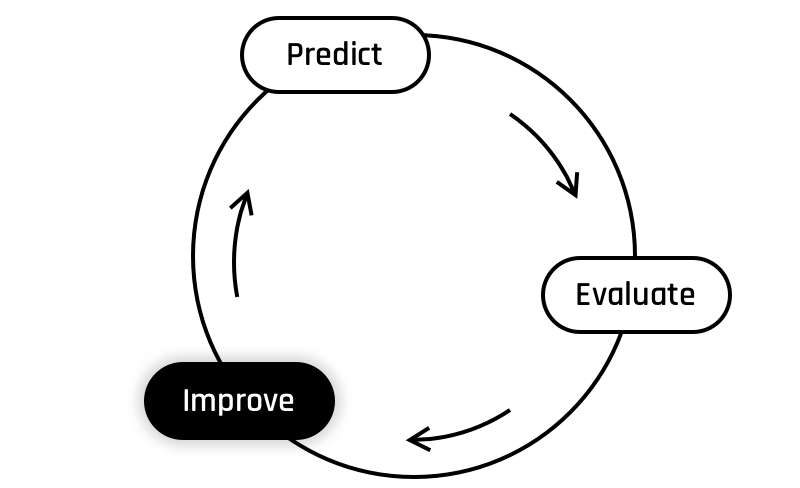
\includegraphics[scale=0.25]{assets/Improve2.png}
\end{figure}

In the previous module, you discovered the first two steps of the learning process:
starting with a model that makes naive predictions and evaluating it.
Now we are going to tackle the third part: improving it!  


Lets take a new dataset:

\begin{figure}[!h]
  \centering
  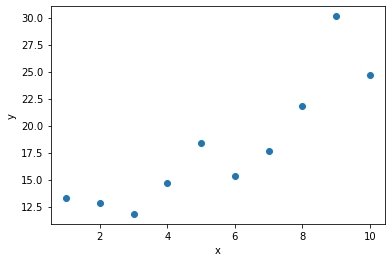
\includegraphics[scale=0.6]{assets/ex03_interlude_plot.png}
  \caption{Scatter plot of a given dataset}
\end{figure}

% =============================== %
\section*{Predict}
% ******************************* %
Given our measure of performance, improvement entails \textbf{reducing the loss (or cost)} measured by the loss function.
If we plot the loss of a model's predictions as a function of its $\theta_1$ parameter (with a fixed value for $\theta_0$), we obtain a curve like this one:
\begin{figure}[!h]
  \centering
  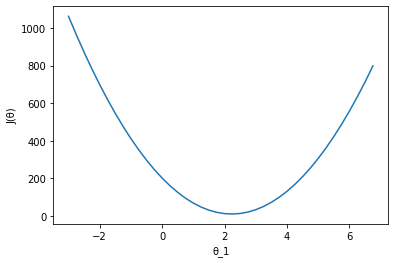
\includegraphics[scale=0.6]{assets/ex03_interlude_cost.png}
  \caption{Loss function given $\theta_1$}
\end{figure}

On the graphs below, you can see that extreme $\theta_1$ values (which modifies the slope of the hypothesis curve - in orange) correspond to a very high loss.
On the other hand, as we get closer to the bottom of the curve, the loss is reduced.  
\begin{figure}[!h]
  \centering
  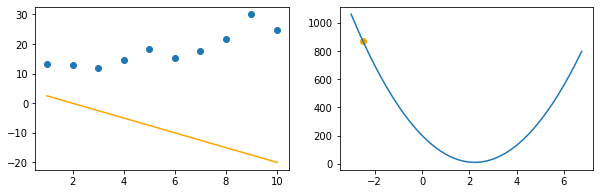
\includegraphics[scale=0.6]{assets/ex03_cost_1.png}
  \caption{A quite bad model}
\end{figure}

\begin{figure}[!h]
  \centering
  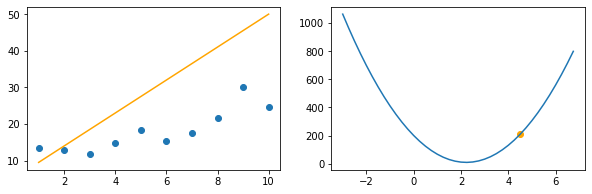
\includegraphics[scale=0.6]{assets/ex03_cost_2.png}
  \caption{A better (but still bad) model}
\end{figure}

\begin{figure}[!h]
  \centering
  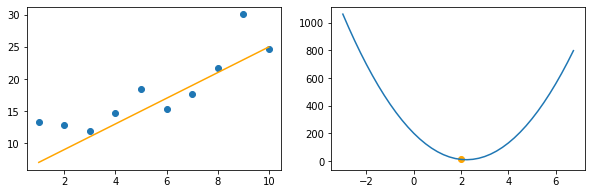
\includegraphics[scale=0.6]{assets/ex03_cost_3.png}
  \caption{A good model}
\end{figure}

The loss function's minimum corresponds to the bottom of the curve.
We want $\theta_1$ to get to this sweet spot.
It means that wherever $\theta_1$ starts at, as the training goes on, it needs to get closer to the value that matches $J(\theta)$'s minimum.


% =============================== %
\subsection*{But how to get closer to the minimum?}
% ******************************* %
Excellent question dear reader.
We're glad you asked!  
First, the algorithm needs to figure out in which direction $\theta_1$ should be moved (i.e. increased or decreased).
It does so by calculating the \textbf{\textit{slope}} of the $J(\theta)$ curve at the current position of $\theta_1$.
If the slope is positive, $\theta_1$ must be decreased.
If the slope is negative, it must be increased.
If you have studied calculus, you probably sense that all of this involves calculating the derivative of the loss function.


The story gets a little more complicated, however, because we have two parameters to adjust: $\theta_0$ and $\theta_1$.
Not just $\theta_1$ (as we showed in our example to simplify).
This means the $J(\theta)$ function doesn't have only one derivative, but two \textbf{\textit{partial derivatives}}.
One that computes the slope of $J$ with respect to $\theta_0$, and a second one for the slope of $J$ with respect to $\theta_1$.
Finally, we package those partial derivatives in a vector of dimension $m$, which is called \textbf{\textit{gradient}} (noted $\nabla$).

Don't worry if you don't master multivariate calculus yet, we have calculated the partial derivatives for you, all you will need to do is write them in Python.  
